\chapter{Projections for the Proposed Measurements}
\label{chap:reach}
In this work we propose to measure the neutron's DVCS beam-spin asymmetry in 
the following two channels:
\begin{enumerate}
   \item Tagged n-DVCS: $D\,+\,\gamma^{*}  \longrightarrow 
      \gamma\,+\,(n)\,+\,p$
   \item Fully exclusive n-DVCS: $D\,+\,\gamma^{*}  \longrightarrow \gamma\,+\, 
      n \,+\,p$
\end{enumerate}

To demonstrate the experimental feasibility and to extract projections for our 
proposed measurements, we present here a simulation study using a realistic 
n-DVCS event generator and the official simulation-reconstruction chain of 
CLAS12 spectrometer upgraded with BONuS12 RTPC. 


\section{Monte-Carlo Simulation}
An event generator for DVCS/BH and exclusive $\pi^0$ electroproduction on the 
neutron inside a deuterium target has been developed \cite{ahmed}. The DVCS 
amplitude is calculated according to the BKM formalism \cite{Belitsky:2001ns}, 
while the GPDs have been taken from the VGG model 
\cite{PhysRevD.60.094017,Guidal:2004nd}. The Fermi-motion distribution is 
calculated with the Paris potential \cite{PhysRevC.21.861}.

The output of the event generator was fed through CLAS12 official simulation 
(GEMC 4.3.0)~\cite{clas12-gemc} and reconstruction (COATJAVA 
5b.7.4)~\cite{clas12-coatjava} chain, to simulate the detectors' acceptance and 
resolutions for all the final state particles, i.e., electrons, photons, 
protons, and neutrons, within the proposed experimental setup of Run Group F.  

\section{Particle Identification}

The final state of neutron Tagged-DVCS event consists of three particles: an 
electron, a proton, and a real photon, while in addition to these particles a 
neutron is required to be detected in the fully exclusive neutron's DVCS 
events. To identify the DVCS events, we first identify the different particles 
of interest. Then, events with three and four detected final-state particles 
will be further filtered by imposing the energy-momentum conservation laws.

For the identification of the different final state particle we use the 
official CLAS12 Event-Builder~\cite{eventbuilder}. In the following subsections 
we revisit the main requirement for the different particles. 

\subsection{Electron Identification} 
For charged particles in the forward detectors, the Event Builder first assigns 
e$^-$ (PID= 11) or e$^+$ (PID= -11) (depending on the bending direction of the 
reconstructed track in the DC) if a particle satisfies all corresponding HTCC 
and ECAL requirements, and has an associated FTOF hit:
\begin{itemize}
 \item 2.0 photoelectrons in HTCC.
 \item 60 MeV in PCAL.
 \item  5-sigma cuts on a parameterized momentum-dependent sampling fraction 
    where "sampling fraction" is ECAL visible energy deposition 
      (PCAL+Inner+Outer) divided by DC momentum.  
      
\end{itemize}

In addition to these initial selections cuts, some regions of CLAS12 have to be 
excluded from the analysis to ensure an accurate detection of the different 
particles. For instance, an electron that hits the edge of the EC will have 
only part of its electromagnetic shower contained within the detector. Also, 
the structure of the torus magnet divides CLAS12 into six separate sectors, 
which makes edge effects non-negligible. Figure~\ref{fig:el_kin} shows the 
kinematic distributions of the DVCS electrons being detected and reconstructed 
in the forward detector of CLAS12 spectrometer in terms of the energy as a 
function of the polar angle ($\theta$) and the azimuthal angle ($\phi$) as a 
function of $\theta$. 

\begin{figure}[tp]
\centering
   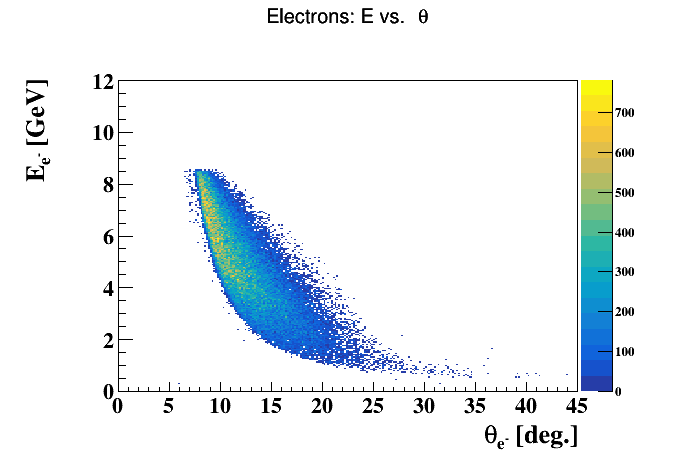
\includegraphics[width=0.48\textwidth,clip,trim=0mm 0mm 0mm 
   20mm]{figs/e_E_theta.png}
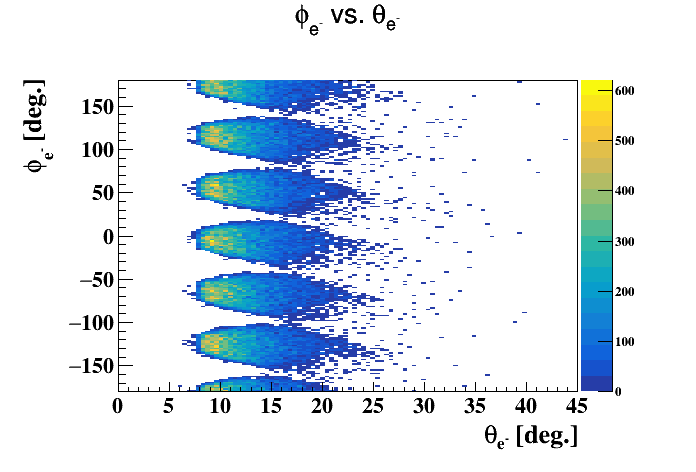
\includegraphics[width=0.48\textwidth,clip,trim=0mm 0mm 0mm 
   20mm]{figs/e_phi_theta.png}
   \caption{Electron's energy as a function of it's polar angle (left) and the 
   azimuthal angle as a function of the polar angle (right), for n-DVCS events.  
   Forward-CLAS12 acceptance and physics cuts are included.}
   \label{fig:el_kin}
\end{figure}
 

\subsection{Proton Identification}
The slow recoiling final state protons will be detected within the BONuS12 
RTPC. As the RTPC is physically within the CLAS12 simulation, but the track 
reconstruction is not finalized yet within CLAS12 reconstruction, we refer to a 
realistic fastmc the reproduces the expected performance of this detector. This 
fastmc has be developed initially from the BONuS6 experiment and tuned very 
precisely after EG6 experimenti \cite{eg6_note}, which have used very similar 
RTPCs.  This fastmc smears the proton's kinematics and applies acceptance 
functions. Regarding the smearing, the momentum, polar angle, azimuthal angle, 
and z-vertex of the protons are smeared with Gaussians using the observed 
tracking resolutions of the RTPC (see chapter 2, section 3 in \cite{eg6_note}).  
For the acceptance, the fastmc:
\begin{itemize}
   \item ensures that the proton's track intersects with the cathode.
   \item removes the tracks which pass in the dead area between the two modules 
      of the RTPC.
\item rejects the track if it goes to the upstream end of the target's holder.
\item applies the RTPC's thresholds on the momentum and the polar angle.
\end{itemize} 
We do not specifically apply energy loss and multiple scattering in our fastmc, 
but we do apply resolution effects based on experimental data that include both 
effects. Figure~\ref{fig:proton_kin} presents the kinematic distributions of 
the recoiling final state protons within the active volume of the BONUS12 RTPC. 

\begin{figure}[htb]
\centering
   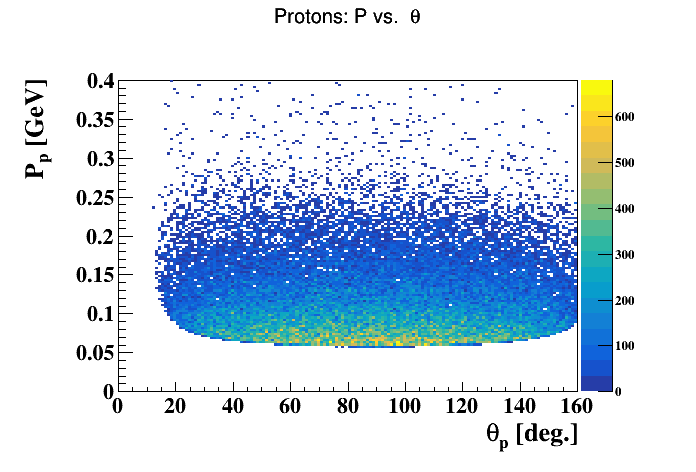
\includegraphics[width=0.48\textwidth,clip,trim=0mm 0mm 0mm 
   20mm]{figs/p_p_theta.png}
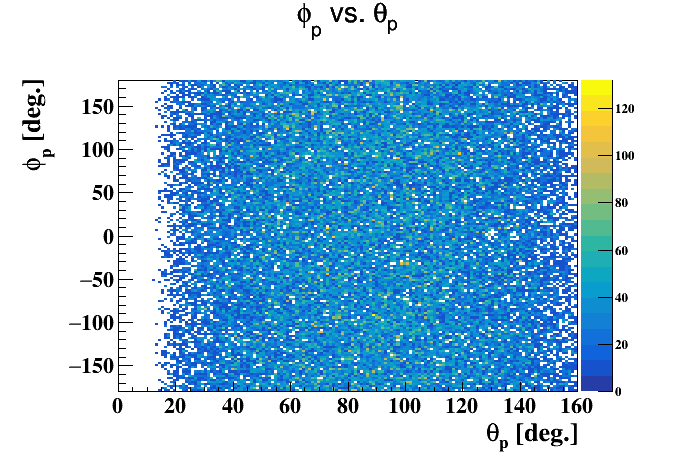
\includegraphics[width=0.48\textwidth,clip,trim=0mm 0mm 0mm 
   20mm]{figs/p_phi_theta.png}
   \caption{Recoiling proton's momentum as a function of it's polar angle 
   (left) and the azimuthal angle as a function of the polar angle (right), 
   from n-DVCS events. BONuS12 RTPC acceptance and physics cuts are included.}
   \label{fig:proton_kin}
\end{figure}
 

\subsection{Neutrals Identification} 

For neutrals, only photon (PID= 22) and neutron (PID= 2112) are considered, and 
particle identification is assigned based on simple beta cut at 0.9. Currently 
only one timing response is used for this, and for ECAL the prioritization is: 
PCAL, EC Inner, EC Outer. The momentum direction is assigned based on the 
neutral's ECAL cluster position and the vertex of the charged particle used to 
determine the start time. For photons, the energy (magnitude of the momentum) 
is calculated from ECAL visible energy and momentum-dependent sampling 
fraction, while for neutrons energy is calculated from beta. For the central 
detector, CND is treated similarly as ECAL, except only neutron PID is assigned 
based on beta and the cut is at 0.8. Figure~\ref{fig:photon_kin} presents the 
kinematic distributions of the neutron-DVCS photons being detected in the 
CLAS12 forward detector. Figure~\ref{fig:neutron_kin} shows similar 
distributions of the detected final state neutrons being detected in both the 
forward and the central detectors of CLAS12 spectrometer. As can be seen from 
figures~\ref{fig:el_kin}, \ref{fig:proton_kin}, ~\ref{fig:photon_kin}, 
~\ref{fig:neutron_kin}, the DVCS electrons and photons are produced very 
forward, which is in a total agreement with out DVCS measurements during the 
6~GeV era of CLAS, while slow recoiling protons are almost emitted flat in the 
polar angle range within the acceptance of the BONuS12 RTPC. The final neutrons 
are mostly emitted above $\theta$ = 40$^{\deg}$, which is outside the 
acceptance of the forward detector of CLAS12 and was the main reason to upgrade 
CLAS12 with the Central neutron Detector during Run Group B to measure the 
neutron DVCS semi-exclusively (E12-11-003).  


\begin{figure}[htb]
\centering
   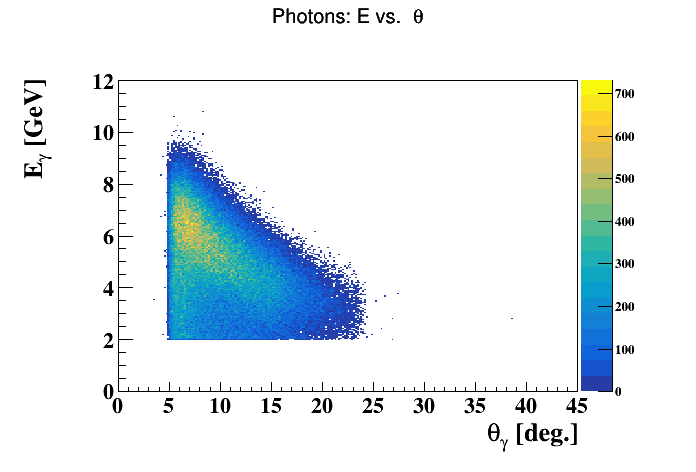
\includegraphics[width=0.48\textwidth,clip,trim=0mm 0mm 0mm 
   20mm]{figs/gamma_E_theta.png}
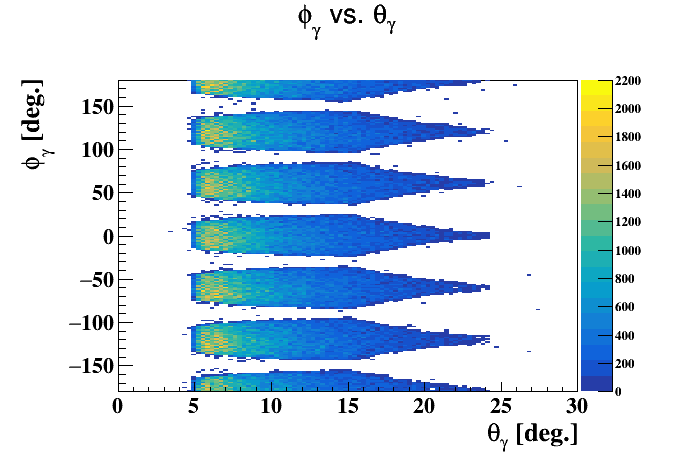
\includegraphics[width=0.48\textwidth,clip,trim=0mm 0mm 0mm 
   20mm]{figs/gamma_phi_theta.png}
   \caption{Photon's energy as a function of it's polar angle (left) and the 
   azimuthal angle as a function of the polar angle (right), for n-DVCS events.  
   Forward-CLAS12 acceptance and physics cuts are included.}
   \label{fig:photon_kin}
\end{figure}
 

\begin{figure}[htb]
\centering
  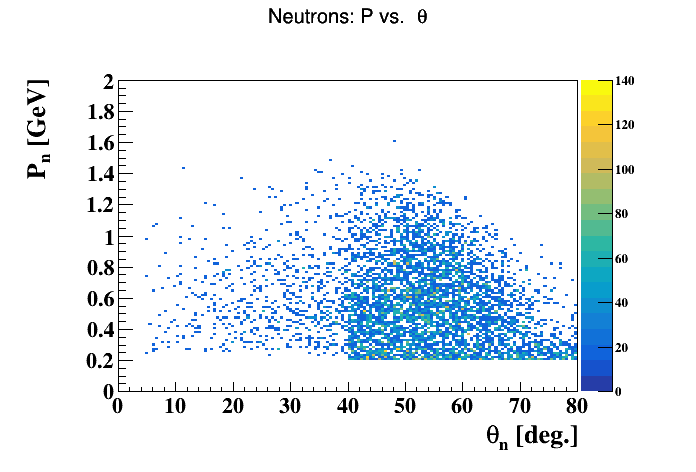
\includegraphics[width=0.48\textwidth,clip,trim=0mm 0mm 0mm 
   20mm]{figs/n_p_theta.png}
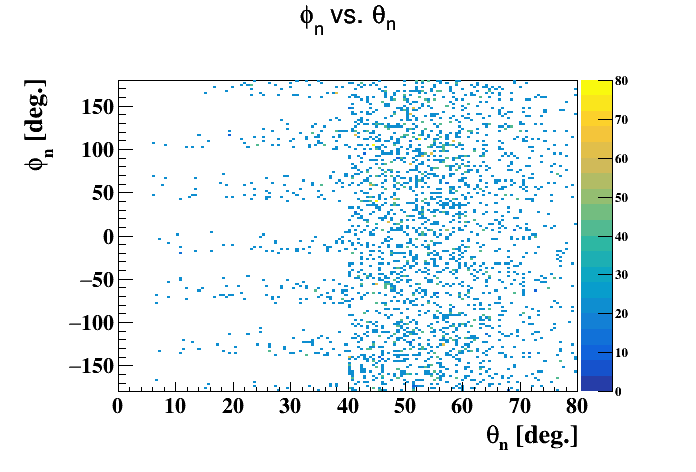
\includegraphics[width=0.48\textwidth,clip,trim=0mm 0mm 0mm 
   20mm]{figs/n_phi_theta.png}
  \caption{Recoiling neutron's momentum as a function of it's polar angle 
  (left) and the azimuthal angle as a function of the polar angle (right), from 
   n-DVCS events. BONuS12 forward and central acceptance and physics cuts are 
   included.}
  \label{fig:neutron_kin}
\end{figure}


\section{Projections}
\subsection{Semi-exclusive selection}
RD to MH: I can help with the conclusions, but you will need to provide first more 
context of the figures. 

\begin{figure}[htb]
  \centering
    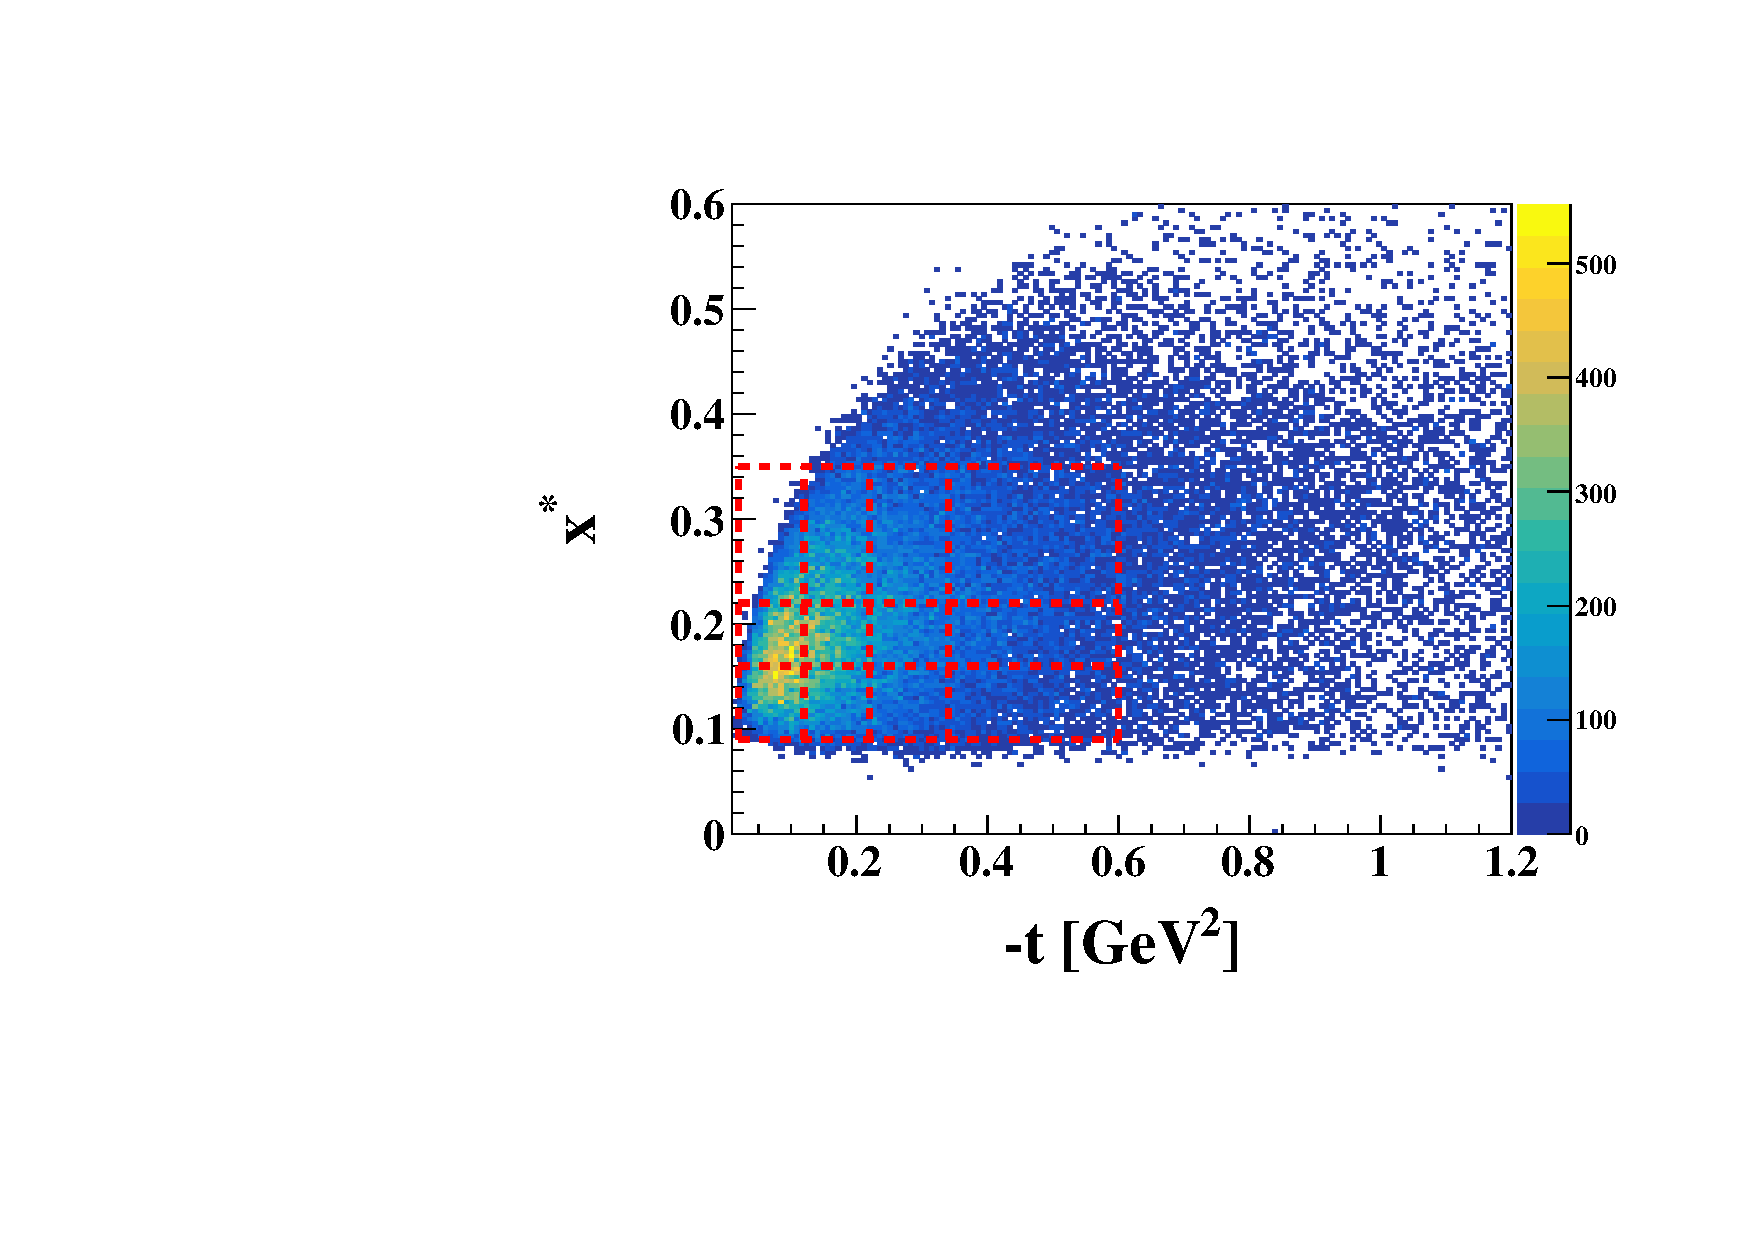
\includegraphics[width=0.55\textwidth,clip]{figs/pdf/t_x*.pdf}
  \caption{Data binning in $x^{*}$ vs $-t$ space.
   \label{fig:binning_x_t}}
\end{figure}

\begin{figure}[htb]
  \centering
    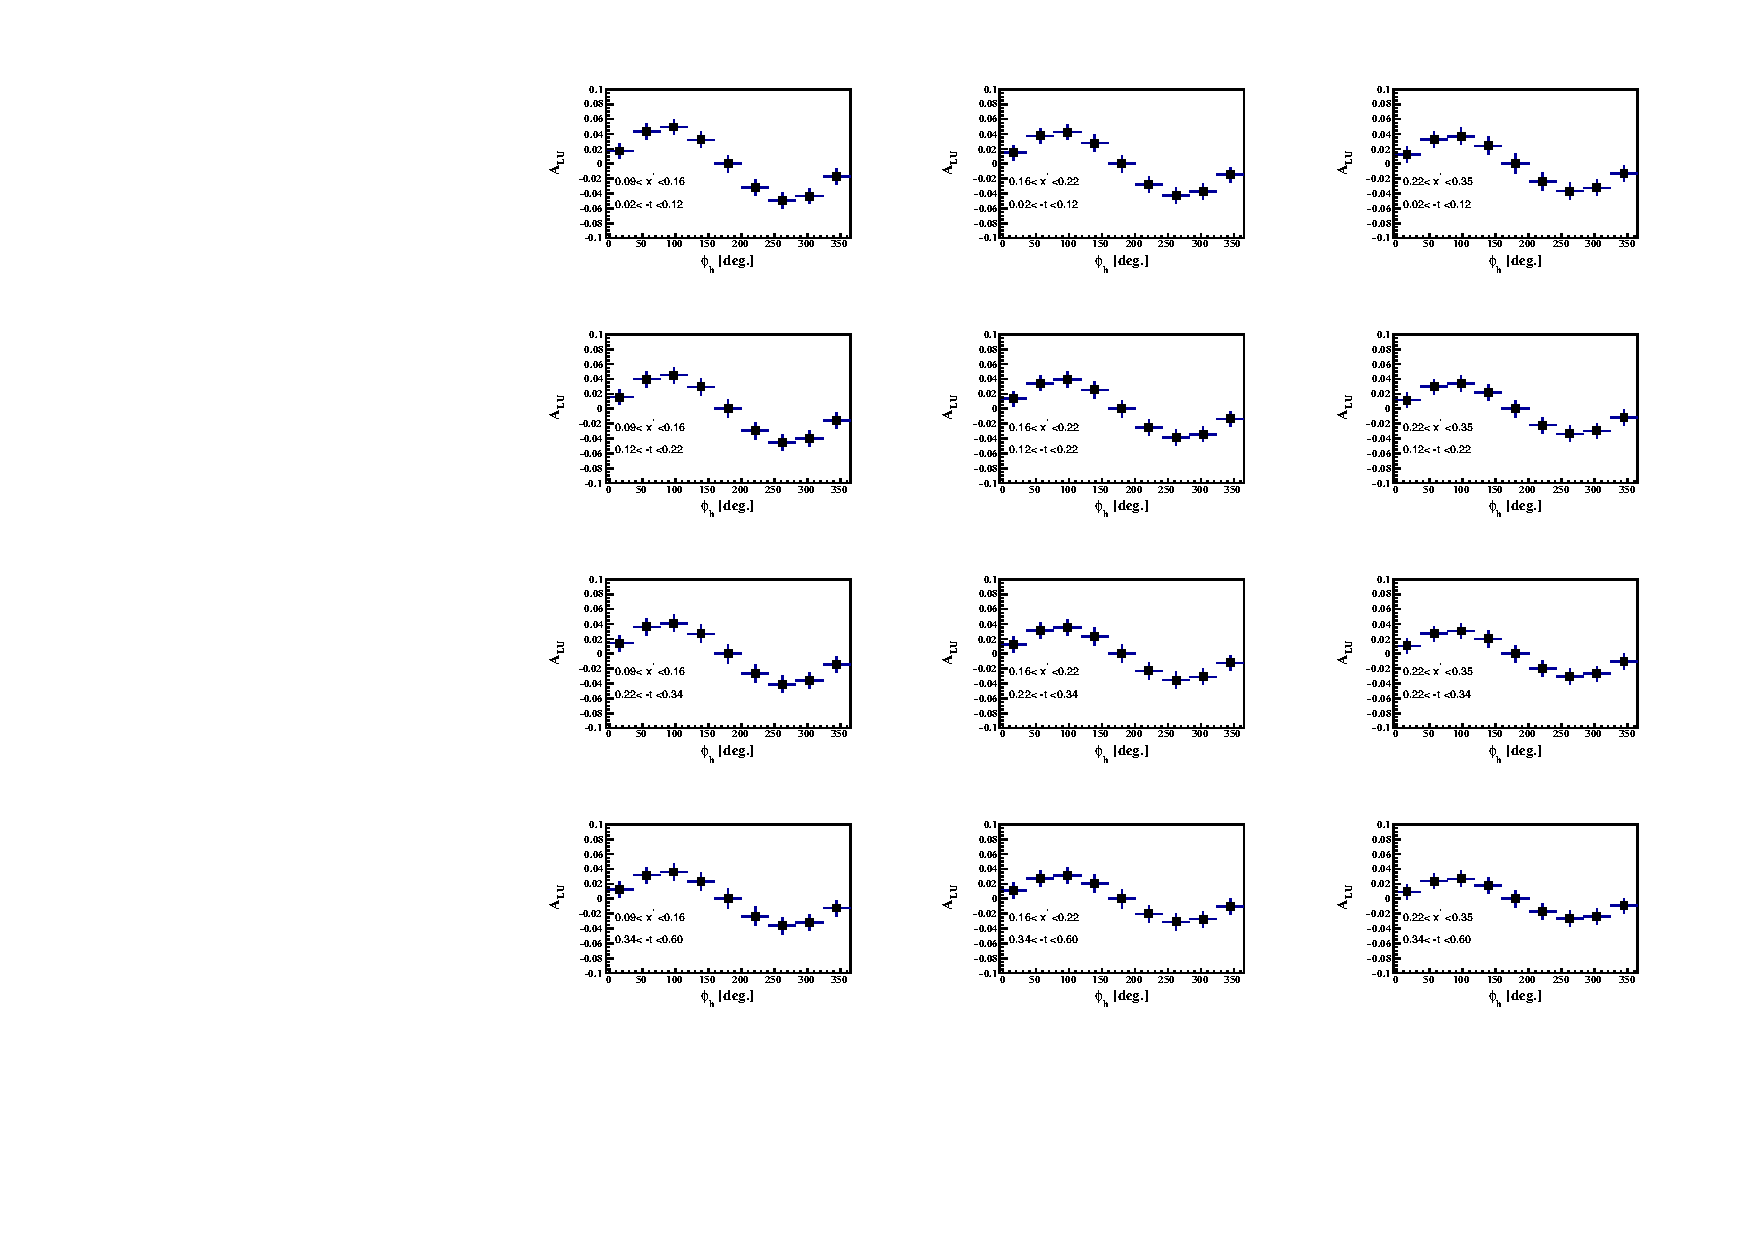
\includegraphics[width=1.1\textwidth,clip]{figs/pdf/BSA_incoherent_Phi_x_t.pdf}
  \caption{Projected beam-spin asymmetries as a function of the hadronic angle 
   $\phi_h$ in the binning of $x^{*}$ vs $-t$ space.
   \label{fig:alu_semi}}
\end{figure}




\subsection{Semi-exclusive selection}
RD for MH: Is this supposed to be Fully exclusive selection?

\begin{figure}[htb]
  \centering
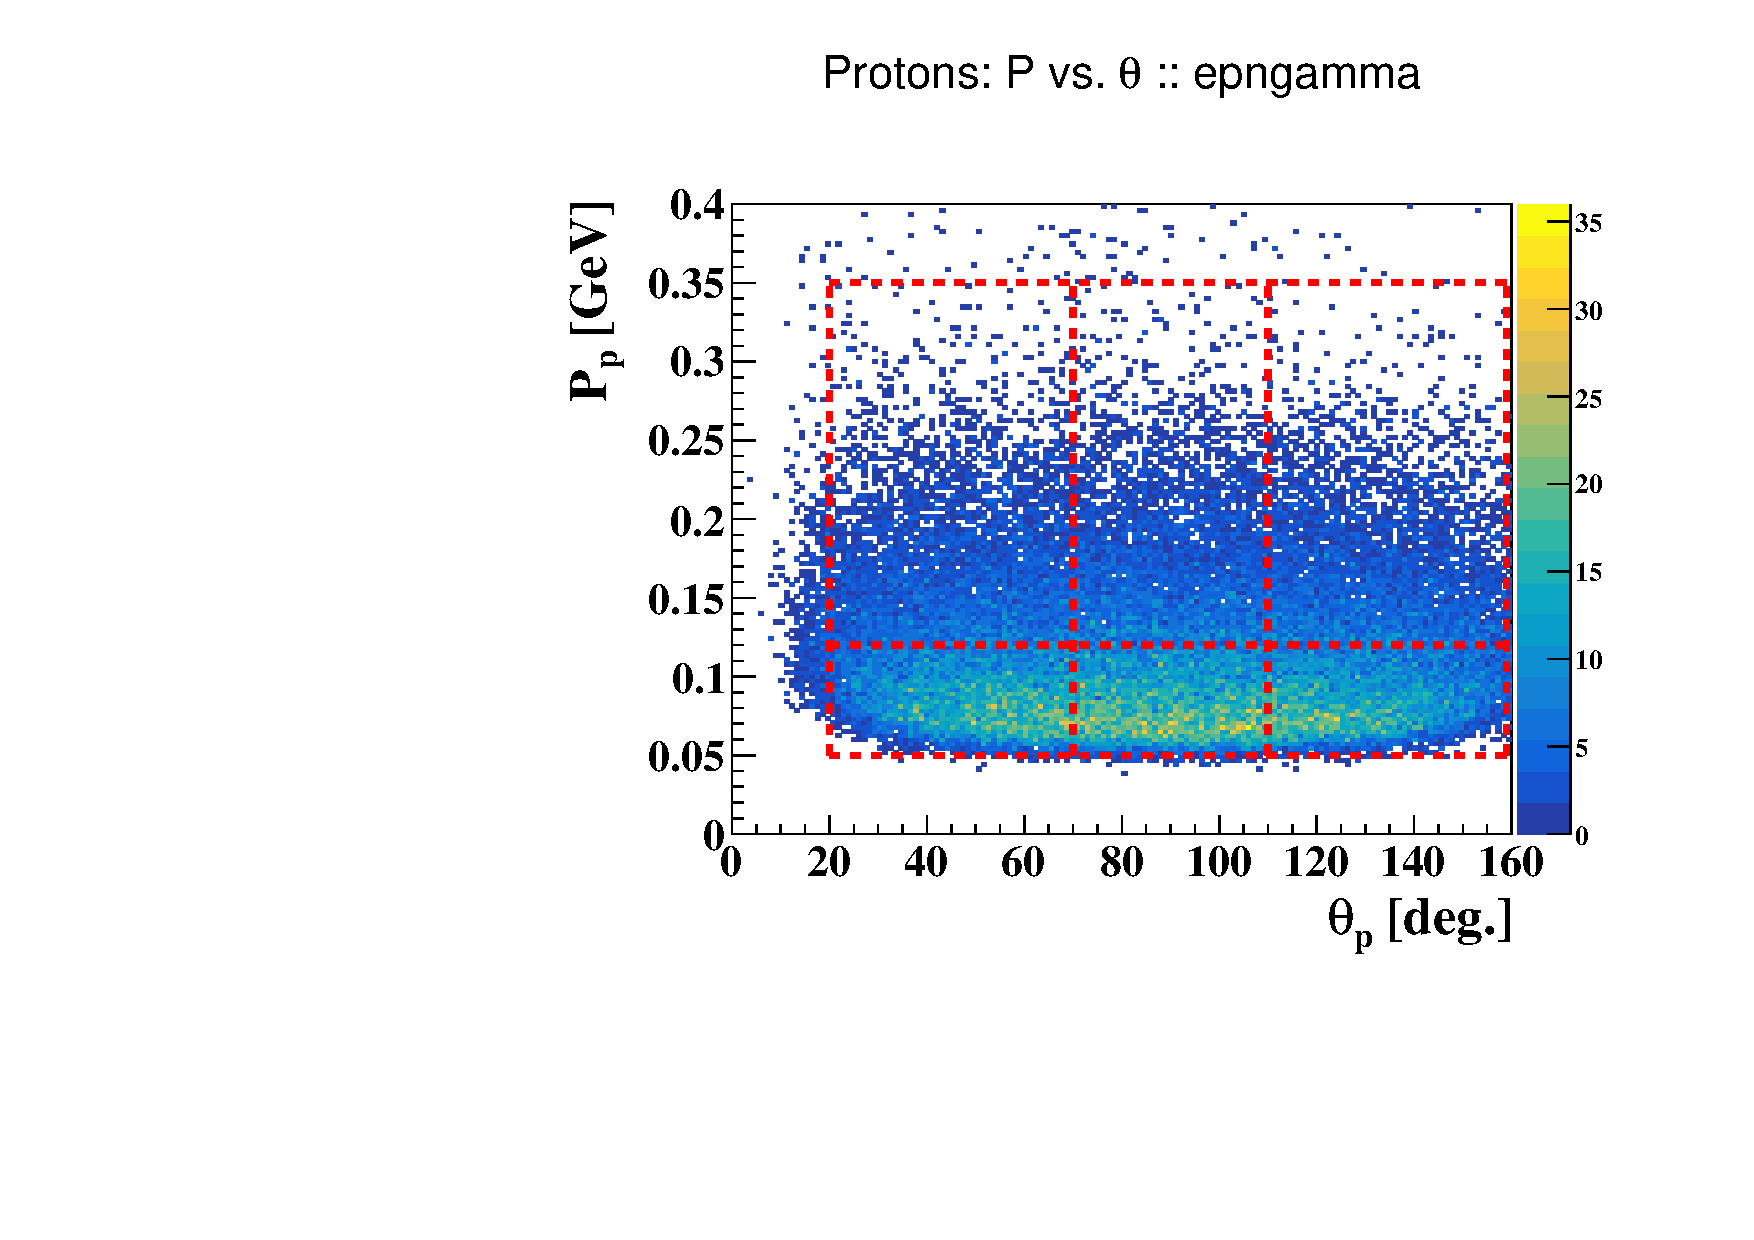
\includegraphics[width=0.55\textwidth,clip,trim=0mm 0mm 0mm 
   20mm]{figs_epngamma/pdf/epngamma_p_p_theta.pdf}
  \caption{Data binning in $p_s$ vs $\theta_s$ space.
   \label{fig:binning_x_t}}
\end{figure}

\begin{figure}[htb]
  \centering
    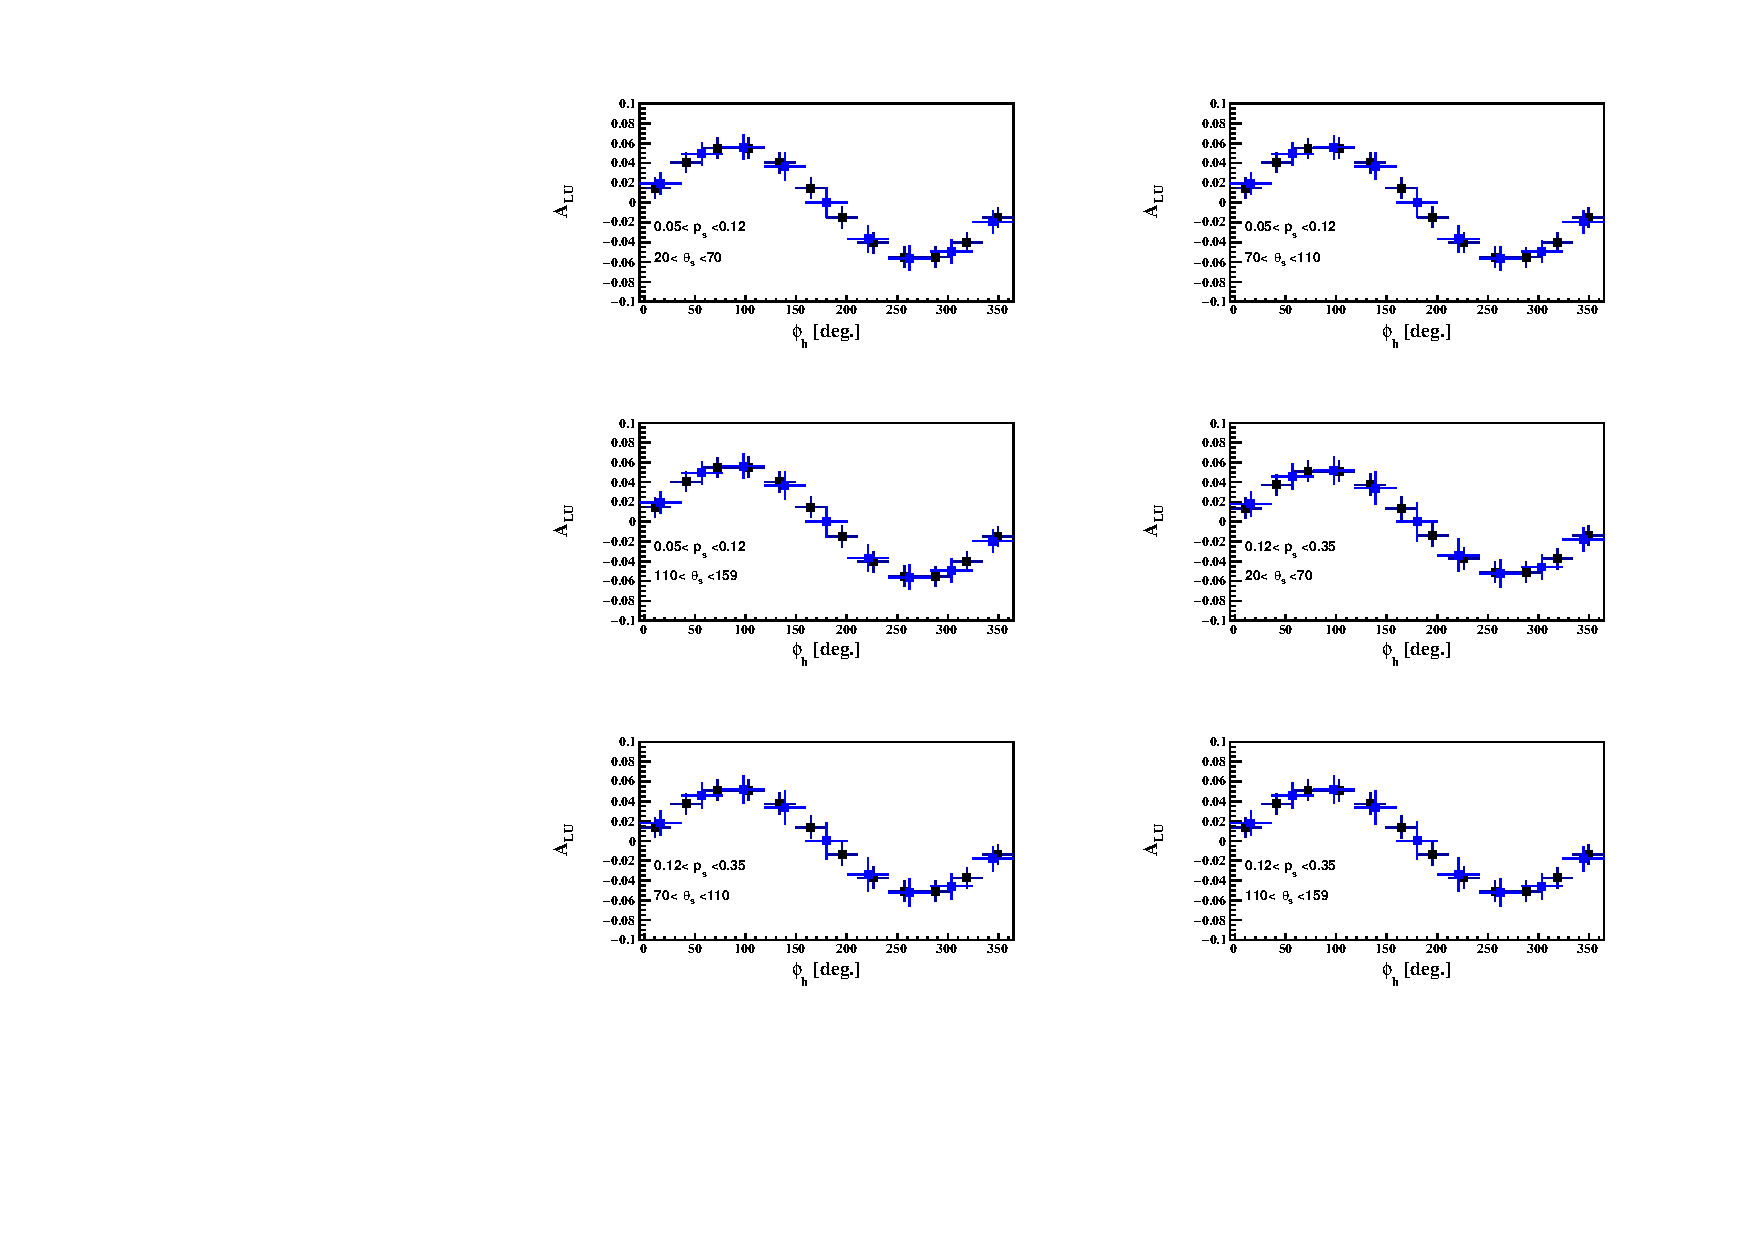
\includegraphics[width=1.1\textwidth,clip]{figs_epngamma/pdf/epngamma_BSA_incoherent_Phi.pdf}
  \caption{Projected beam-spin asymmetries as a function of the hadronic angle 
   $\phi_h$ in the binning of $p_s$ vs $\theta_s$ space.
   \label{fig:alu_semi}}
\end{figure}



